\documentclass{sigchi-alternate}

% Use this command to override the default ACM copyright statement (e.g. for preprints). 
% Consult the conference website for the camera-ready copyright statement.
%\toappear{%
%Permission to make digital or hard copies of all or part of this work for personal or classroom use is granted without fee provided that copies are not made or distributed for profit or commercial advantage and that copies bear this notice and the full citation on the first page. Copyrights for components of this work owned by others than the author(s) must be honored. Abstracting with credit is permitted. To copy otherwise, or republish, to post on servers or to redistribute to lists, requires prior specific permission and/or a fee. Request permissions from \href{mailto:permission@acm.org}{Permissions@acm.org}.\\[3pt]
%\textit{CHI 2014}, April 26--May 1, Toronto, ON, Canada.\\
%Copyright is held by the owner/author(s). Publication rights licensed to ACM.
%}
%\submissionversion{CHI 14}

% Load basic packages
\usepackage{balance}  % to better equalize the last page
\usepackage{graphicx} % for EPS, load graphicx instead
\usepackage{url}      % llt: nicely formatted URLs
\usepackage[utf8]{inputenc}

% llt: Define a global style for URLs, rather that the default one
\makeatletter
\def\url@leostyle{%
	\@ifundefined{selectfont}{\def\UrlFont{\sf}}{\def\UrlFont{\small\bf\ttfamily}}}
\makeatother
\urlstyle{leo}

% remove those two lines if you don't want to use biblatex
\usepackage[style=sigchi,backend=biber,doititles]{biblatex}
\addbibresource{references.bib}
%\DeclareBibliographyCategory{ignore}
%\addtocategory{ignore}{AGORAVA}
%\addtocategory{ignore}{CLOUDRAIL}
%\addtocategory{ignore}{SOCIALMEDIA-ABSTRACTIONS}
%\addtocategory{ignore}{ASNE}

% hyperref was already loaded by the documentclass.
% Use nohyperref option to prevent this from happening.
\hypersetup{
	pdftitle={Ingen titel än},
	pdfauthor={LaTeX},
	pdfkeywords={SIGCHI, proceedings, archival format},
	bookmarksnumbered,
	pdfstartview={FitH},
	colorlinks,
	citecolor=black,
	filecolor=black,
	linkcolor=black,
	urlcolor=black,
	breaklinks=true,
}

% create a shortcut to typeset table headings
\newcommand\tabhead[1]{\small\textbf{#1}}

% End of preamble. Here it comes the document.
\begin{document}

% Arabic page numbers for submission. 
% Add this line to eliminate page numbers for the camera ready copy
%\pagestyle{empty}

\title{Ingen titel än}

\numberofauthors{2}
\author{
	\alignauthor{Fredrik Jonsén\\
		\affaddr{Linköping University}\\
		\affaddr{Linköping, Sweden}\\
		\email{frejo105@student.liu.se}}
	\alignauthor{Alexander Stolpe\\
		\affaddr{Linköping University}\\
		\affaddr{Norrköping, Sweden}\\
		\email{alest170@student.liu.se}}
}

% Teaser figure can go here
%\teaser{
%  \centering
%  \includegraphics{Figure1}
%  \caption{Teaser Image}
%  \label{fig:teaser}
%}

\maketitle

\begin{abstract}
Coming later
\end{abstract}

\section{Introduction}
Today a lot of people are using social media in one way or another and it is estimated that there will be around 2.67 billion social media
users around the globe by 2018\autocite{STATISTA_SN_WORLD_USERS}. Most of these social networks have released Application Programming Interfaces (APIs)
which developers can utilize to integrate these networks into their software.

Social network usage is growing and has gone from 0.97 billion users in 2010 to 2.14 billion in 2015.\autocite{STATISTA_SN_WORLD_USERS}. This would
account for approximately 29\% of the earth's population in 2015, which was 7.347 billion 2015\autocite{WORLD_BANK_POPULATION}. It is worth noting
that this counts created user accounts and not unique users, one person can have several accounts over multiple networks, and accounts may not
belong to an actual person, but rather companies, organizations, or bots.

Because of the currently high, and still growing, number of social media users we find it highly likely that we will see an increasing number of
applications that involve social media in their software in one way or the other. Out of all the social networks existing today there are twenty
that have more than 100 million active accounts\autocite{STATISTA_LEADING_SOCIAL_NETWORKS}. This means that if one would want to create an application
that involves a lot of social networks we will have to do a lot of work just to implement all of these into our system.

\subsection{Purpose}
Because of this we see a need for a way to combine these social network APIs in some way to save development
time and reduce the amount of duplicate code written in software. The purpose for this project is to create a library 
that combines the APIs in a modular fashion, where each API serves as a module in order to simplify adding new networks,
and make it easier to involve social media in software. 

A software library by definition is a set of pre-written code that a developer might add to a project in order to add more functionality or to ease the 
development process\autocite{TLDP_LIBRARY_DEFINITION}. 

For our study, we define modularity as the extent to which a program can be divided into modules where\autocite{Kiczales:2005:APM:1062455.1062482}:
\begin{itemize}
	\item Each module has a well-defined interface that describes how the system can interact with it.
	\item Changes to the underlying functionality of a module does not affect the modules interface.
	\item Modules can be put together with other modules in different ways to make a complete program
\end{itemize}
In our case modularity will mostly affect how easy it will be to integrate new social media APIs in the future.

Over time, as new Social Networks enter the market, it will have to be possible to integrate them into our library. As such, the code will have to be maintainable.
Maintainability is a very broad term, but in general focuses on how simple the code in itself is to work with, when changes or new additions are necessary.
In the Theory chapter we will explore this subject more thoroughly. For the evaluation of the maintainability of our library, we will be making using of the third
party tool SonarQube\footnote{https://www.sonarqube.org/}.


\section{Research Question}
Is it possible to create a maintainable modular library for Social Network APIs?

As the question pertains to the \textit{possibility} of creating the library, it is also necessary to define what would make us deem it impossible to finalize
the library with a satisfactory result. In regards to this, we see two major potential risk factors:
\begin{enumerate}
	\item It may not possible to generalize the results of the APIs, but each API will instead require a large mount of exceptions, making a common interface meaningless.
	\item The rate of changes to the APIs may be unmaintainable. If we during the course of the relatively short development time find ourselves having to go back multiple
	times to adjust already implemented functionality due to changes in the API, we will consider the library unmaintainable.
\end{enumerate}
\section{Limitations}
Because there are so many social networks existing today and we have a finite amount of time to complete this
project we will focus on a smaller set of APIs to implement into our library.  We have set up a few criteria 
for the APIs so we can find suitable candidates for our library, which are:
\begin{itemize}
	\item The social network must be one of the 22 most popular\autocite{STATISTA_LEADING_SOCIAL_NETWORKS}.
	\item It must be relevant for our geographical location, in this case Europe.
\end{itemize}
Other than this we will judge the API itself subjectively by how good its documentation is, its functionality and its ease-of-use. 

\section{Theory}
\subsection{Code Reuse}
A lot of time and money can be saved by reusing code, of which libraries are one form. Although there are
some issues with using libraries, the gains from avoiding reinventing the wheel makes writing and using
libraries a common practice, in particular in open source software\autocite{2998479020080101}.

Writing code which can be easily reused requires a deeper analysis of the problem domain, which may increase the cost and time required compared 
to developing the same code without reuse in mind, but can drastically decrease the cost of developing systems in the future where the code can 
be reused \autocite{lim1994effects}. This cost reduction is apparent foremost in terms of direct cost of development, but also in time-to-market, 
which can be argued to be even more important in the long term\autocite{griss1993software}.

With code reuse there are also several potential issues which have to be kept in mind, both when it comes to the implementation itself but also 
when it comes to using the implementation. Backwards compatibility between versions is a major topic in itself\autocite{raemaekers2012measuring}. There 
is also the risk of a library being abandoned by it’s maintainer. This is especially true for proprietary libraries, where the source code may not 
be available. It this case, the library might have to be replaced, making all the effort to use the library wasted.

\subsection{Library Interface Design}
When designing our library we will want keep several things in mind. We want to design the library so it’s easy and straightforward to use for a 
developer. As Henning points out in his article\autocite{Henning:2007:ADM:1255421.1255422}, about design of APIs, it is very easy to create a bad one, 
but very hard to create an API that feels natural and easy to work with. APIs, as we know, are a kind of interface for a program to gain access to 
another program without direct access, and can be compared to the interface of our library.

Henning continues to discuss guidelines for how an API should generally be designed. What feels most relevant to our work is how 
he describes how the APIs should be designed from the perspective of a user, because when it’s done from the implementer's point of view the 
needs of the user are often forgotten. It’s usually best to document first, because when it is done after the implementation the programmer, who 
wrote the functionality, will usually just dictate what he did, rather than make it is obvious enough for others who are not as familiar with the code.

\subsection{Maintainability}
Maintainability can be defined as the simplicity with which defects can be corrected and the library can be extended or modified to support future 
requirements.\autocite{5733835}. This can generally be measured by certain quantifiable attributes, such as unit test coverage, lines of code and cyclomatic complexity.
\autocite{SONARQUBE_MAINTAINABILITY_DEFINITION}. It also includes more subjective aspects, such as how self-explanatory the code is, and how well commented sections
of necessarily complex code is.

\subsection{Social Media APIs}
A social media API is an interface through which the software can integrate functionality offered by the social media platform, commonly set up as a REST API. 
These can be used through registering the application on the social media site, thus acquiring an authentication token which can be used to call different
endpoints via HTTP. The services offered varies between the APIs, but tend to share some basic functionality such as publishing posts and sending private messages.

As mentioned, one of the biggest issues with using libraries is the risk of the project being abandoned. This risk increases significantly when the library
itself uses APIs which integrate oft-changing platforms, such as the case of Social Media. The rate of change differs between networks, in some cases on average
three times a year\footnote{https://developers.facebook.com/docs/apps/changelog}, in other cases several times a month\footnote{https://www.hitchhq.com/twitter/activities},
although the impact of the changes varies greatly. At best, a lack of active development simply means missing out on new functionality. In other cases, such as 
unfixed security vulnerabilities\footnote{https://github.com/gorbin/ASNE/issues/107}, may render the library unusable.

\subsection{Similiar work}
Several similar works, Agorava\footnote{http://www.agorava.org/}, ASNE\footnote{https://github.com/gorbin/ASNE} and 
SocialMedia Abstractions\footnote{https://github.com/socialsensor/socialmedia-abstractions} serve the same or similar purposes, but all were abandoned before reaching a 
stable release. In the case of ASNE, the project was abandoned explicitly due to a lack of free time. This shows the issue of a library having only a single maintainer, 
as the project risks being abandoned by it's developer as soon the project is no longer a priority. The others have no stated reason for the lack of continued development.
There are also commercial services\footnote{https://cloudrail.com} which provide this functionality for some popular APIs, but charge money to sign up 
and use. As it is proprietary it's inner workings are completely opaque, and thus will not be examined by this study.

\subsubsection{Encountered issues}
Despite being abandoned, we hope to still learn from the problems the similar libraries encountered and solved. For this, we looked into each project's issue
tracking (where available) and commits. This was somewhat complicated in that one project, SocialMedia Abstractions, simply had not used issue tracking. 
Another project, ASNE did use issue tracking, but much of the discussion regarding individual issues was largely in Russian, making it unusable in our case. 
The issues, despite the name, did not always regard bugs. In the vast majority of cases, issued stemmed from users misunderstanding the library documentation,
requesting features, or suggesting refactoring of code to increase maintainability. In the case of documentation misunderstandings, these were often
solved by simply adding examples. There was also a noticeable difference in the amount of issues pertaining bugs in ASNE, which included no automatic tests,
compared to Agorava, which includes a large amount of automatic tests, and had almost no issues regarding logical errors, despite having a much larger code base.

\section{Method}
To find out if we could create a modular library for social network APIs we structured our project into three different parts. We began with evaluating the most 
popular networks on a basis of which are relevant for our project and which are appropriate to integrate into our library based on functionality. We then implemented
the library, using SonarQube throughout development to ensure code quality and maintainability stayed high. Lastly we evaluated the library in two different ways.
First we analyzed the data we got from SonarQube and see how well our library performs, and then attempted to integrate our library into an existing application, 
Blixtvakt\footnote{http://www.blixtvakt.se}, in order to test its practical usability.

\subsection{Social Networks selection}
To choose which APIs to implement into our library we initially looked at what social media network sites where most popular\autocite{STATISTA_LEADING_SOCIAL_NETWORKS}.
Out of these networks we sorted out those which were geographically irrelevant for the focus of this project, which is the European market. We then further narrowed down
the list by looking at the functionality of each API. We selected the APIs which shared a lot of common functionality, which made them more appropriate for the core idea
of our study, to develop a modular library.

\subsection{Implementation}
When we had chosen APIs to implement we started we started to implement our library. For this we have chosen to work in the Java language, as we in our evaluation will be 
integrating our library with the backend of Blixtvakt. We used the most current version of Java at the time of our project, Java SE 8.  We used several tools, which we will
describe briefly.
\subsubsection{Maven}
Maven\footnote{https://maven.apache.org/} is a project management tool. While the tool includes a lot of functionality, we mostly made use of its automated build tool, release-, and
dependency management.
\subsubsection{IntelliJ IDEA}
IntelliJ IDEA\footnote{https://www.jetbrains.com/idea/} is the Integrated Development Environment we chose for our project. It offers integration with Maven, syntax highlighting,
static analysis, boilerplate code generation and other functionality to simplify the implementation work.
\subsubsection{Travis CI}
Travis\footnote{https://travis-ci.org/} is a free Open Source service for continuous integration. It integrates with github and runs tests automatically for the project when changes are
checked in. When done, participants of the project can be notified of the result.
\subsubsection{SonarQube}
Sonarqube\footnote{https://www.sonarqube.org/} is a service for, in their own words, continuous code quality. As with Travis, it integrates with GitHub and automatically runs a series of
checks when code is committed to the repository. This includes analysing the code for general issues, such as a high cyclomatic complexity, missing documentation and dead code, but also
more detailed issues which may be easy to miss, such as potential infinite loops, unhandled exceptions, or checking floating point numbers for equality.

\subsection{Work Method}
We chose to work using a test driven development process, where we first wrote tests for our interfaces. During this process we also documented the functionality according to 
Hennings\autocite{Henning:2007:ADM:1255421.1255422} concept of documenting first, in an effort of making the documentation more understandable from the users perspective. During this
period we implemented functionality iteratively for our chosen APIs, implementing one functionality at a time for each as to not be left with only one fully implemented API in our library.

\subsection{Design}
\begin{figure}
	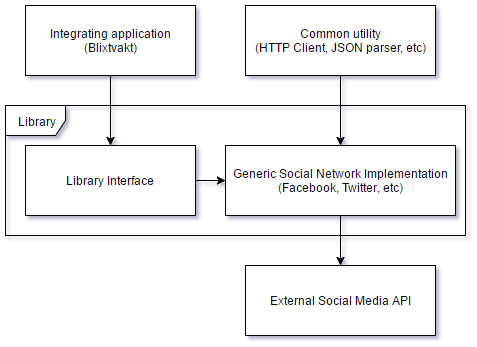
\includegraphics[width=\columnwidth]{LibraryImplementation.png}
	\caption{Architectural overview of library and use case}
	\label{fig:architecturalOverview}
\end{figure}
Our library mainly consist of two parts, see figure~\ref{fig:architecturalOverview}. Where the library interface is what the users are in contact with when interacting with our library. This interface is an abstraction
of a generic social network API. The Generic Social Network Implementation is the actual implementation of each social media platform and acts as the middleware between the interface and the 
external social media platforms.
The internals of each implementation might differ greatly, where some already had an existing library that we could plug in and use for our library, while we had to implement others completely
ourselves, using the REST APIs directly. The ones we implemented use common utility tools such as an HTTP client and a JSON deserializer in order to be able to properly communicate with the external
platforms.

The already existing libraries we used are:
\begin{itemize}
	\item twitter4j (http://twitter4j.org/)
	\item facebook4j (https://facebook4j.github.io/)
	\item jumblr (https://github.com/tumblr/jumblr)
\end{itemize}

\subsection{Evalution}
The evaluation of our library consists of two parts. Throughout the project we have used SonarQube to analyze the quality and maintainability of our code, which is the first part. The second part
involves integrating our library into the backend of Blixtvakt, which is an mobile application that warns users about lightning strikes in a given area chosen by the user. This will give us a more
hands-on experience on how easy our library is to use in practice and the more analytical aspect gained from the SonarQube analysis. 

When integrating our library into into Blixtvakt we will mainly focus on if we feel that there is anything lacking, or if something is not working as intended. If we feel the need to go back and
change the source code of the library or change its interfaces our library is deemed unsatisfactory. 


\balance

% If you want to use smaller typesetting for the reference list,
% uncomment the following line:
% \small

% If you don't want to use biblatex uncomment the following two lines and remove the one after
%\bibliographystyle{acm-sigchi}
%\bibliography{sample}
\printbibliography[notcategory=ignore]

\end{document}
